\documentclass[5p]{elsarticle}
\usepackage[hypcap]{caption}
\usepackage{float}
\usepackage[hidelinks]{hyperref} 
\usepackage{natbib} 
\setcitestyle{bracket}
\setcitestyle{authoryear}
%\setcitestyle{comma}
\setcitestyle{sort}

\usepackage{subcaption}
\usepackage{url}

\begin{document}
\begin{frontmatter}
\title{Creating updated, scientifically-calibrated mosaics for the RC3 Catalogue}
	\begin{abstract}
The Third Reference Catalogue of Bright Galaxies (RC3) is a reasonably complete listing of 23,010 large, bright galaxies. Using the latest Sloan Digital Sky Survey's  Data Release 10 (SDSS DR10) data, we provide  color composite images and scientifically-calibrated FITS mosaics in all SDSS imaging bands, for all the RC3 galaxies that lie within the survey's footprint. To get a larger sky coverage, we then conduct the procedures on  photographic plates taken by the Second Palomar Observatory Sky Survey (POSS-II) for  the B, R, IR bands. Due to the positional inaccuracy inherent in the RC3 catalog, the mosaicking program uses a recursive algorithm for positional update first, then conduct the mosaicking procedure using IPAC's Montage.The program is generalized into a pipeline, which can be easily extended to future survey data or other source catalogs.
	\end{abstract}
\end{frontmatter}
\section{Introduction}
Astronomical catalogs such as the famous Messier Catalog and New General Catalog (NGC) has its historical usage in helping  astronomers  study objects that shares some common property. This was particularly important in the days when all-sky information was not available, so data was taken by pointing the telescope at some particular location.  
Large sky surveys such as the Sloan Digital Sky Survey(SDSS), the Second Palomar Observatory Sky Survey (POSS-II), and Two Micron Sky Survey (2MASS) not only provide improved astrometry for finding these objects, but also photometry and systematics information that could affect the imaging of the detected sources, such as information generated through SDSS's $\texttt{photo}$ pipeline (\citealp{photopaper}).
With large sky surveys such as the SDSS, the job of target-based imaging is much  easier because the position values of objects of interest are readily accessible via NED/ SIMBAD. The role of the astronomical catalogue has evolved into samples for statistical studies for some particular type of object (QSO, pulsars, x-ray sources) or used as targets in cosmology studies.
\\
\indent
There has been existing literature on making mosaics for galaxies that lies inside the Third Reference Catalog of Bright Galaxies  (RC3) using data from SDSS. Hogg and Blanton made g,r,i colored images of selected RC3 galaxies by using data from the SDSS Data Release (DR)6.\footnote{\url{http://cosmo.nyu.edu/hogg/rc3/}} The EFIGI catalog (\citealp{efigi}), dedicated to studying morphology of galaxies, also  obtained a subset of 4458 RC3 FITS and color images using SDSS DR4 data and discarded artifacted or missing data via visual inspection. We performed the mosaicking procedures on the whole RC3 catalog using an automated positional update algorithm on the most recent SDSS DR10 imaging data. In addition, we designed a mosaicking pipeline that creates scientifically-calibrated mosaics, color-band images, as well as a set of updated positions, which can be easily adapted for existing surveys such as 2MASS, POSS-II, or future imaging data release from  Dark Energy Survey (DES) or the Large Synoptic Survey Telescope (LSST) for larger sky coverage and multi-band images.
\section{The RC3 Catalog and Survey Data}
The attempts to select catalog object based on brightness selection limits traces back to the original Harvard Survey of External Galaxies (H. Shapley and A. Ames 1932) which contained 1249 objects brighter than the 13th magnitude. Many of these were included in the University of Texas monographs in astronomy, predecessors to the  RC3 catalog .The RC3 Catalog is an update of the Original and Second Reference Catalog of Bright Galaxies, which collected from 150 different sources, each telescope has different accuracy, precision, and coverage. The RC3 compiled by \citealp{rc3}, contains a  complete listing of 23,010 galaxies with $D_25$ apparent major isophotal diameter  greater than 1 arcminute and with a total B-band magnitude greater than 15.5 nanomaggies. After the RC3 catalogue was published, it was incrementally updated from any available data and maintained by Harold G. Corwin.\footnote{http://haroldcorwin.net/rc3/bugs.rc3} Since imaging data used to update these sources came from various different imaging program and telescopes, there was a non-uniform distributed of updated galaxies. In this project, we used the catalogue information available through the VizieR Service  which contained the original  RC3 data published in 1991. There is also a 1994 version updated by Corwin available on VizieR. 
\\
\indent  Since the RC3 catalog  is a reasonably complete representation of large, bright nearby galaxies in the extragalactic sky, its usage is still evident in literature. Selected galaxies or complete subsets are used in astrophysical studies of  quasars and X-ray sources(\citealp{xray}) or  galaxy morphology and properties.  The RC3 catalog is also used in statistical studies  for cosmology studies such as the New York University-Value Added Galaxy Catalog (\citealp{nyuvagc}).
\subsection{Positional Inaccuracy in RC3 Catalog}
	\label{sec:position}
	The principle motivation behind the automation algorithm is to resolve the problem of centering galaxies and finding RC3 galaxy in a given field of view. Initially, using the standard mosaicking steps in Montage, we obtained many images with  off-centered or missing galaxies due to the inherent inaccuracy of the positions in the catalog. There is an non-uniform update of the catalog after the catalog was publish, more accurate position was collected from whatever sources and data available. The B2000 coordinates in the FK4 frame of  RC3 galaxies are denoted with two different levels of accuracy: HH MM SS.s, DD MM SS for the positions that has been updated  with accuracy of about 5-8 arcsec and  HH MM.m, DD MM for galaxies whose positional accuracy remain  1-2 arcminutes as in the original catalog.  In the 1991 version of the catalog (\citealp{rc31991}), there still remains 5492 RC3 galaxies that fall in the latter group.
\subsection{Data}
%\begin{figure*}[!hbt]
%\center
%%\begin{table}
%    \begin{tabular}{|l|l|l|l|}
%    \hline
%    ~                         & SDSS          & 2MASS              & POSS-II             \\ \hline
%    Imaging bands             & Optical g,r,i & Near-infared J,H,K & Optical R, B,IR     \\ \hline
%    Sky Coverage              & 35.28\%       & 99.998\%           & 78.27\%              \\ \hline
%    Resolution (arcsec/pixel) & 0.396         & 2.0                & 1.7                 \\ \hline
%    Imaging Technique         & CCD           & Infared array      & Photographic Plates \\ \hline
%    
%    \end{tabular}
%    
%%\end{table}
%\caption{Comparison of survey and telescope specifications }
%\end{figure*}
\begin{table}
\footnotesize
    \begin{tabular}{llll}
    \hline
    ~                           & SDSS    & 2MASS         & POSS-II             \\ \hline
    Imaging bands               & g,r,i   & J,F,K         & R, B,IR             \\
    Sky Coverage(\%)                & 35.28 & 99.998      & 78.27             \\
    Resolution($^{\prime\prime}$/pix) & 0.396   & 2.0           & 1.7                 \\
    Imaging Technique           & CCD     & Infared array & Photographic Plates \\ \hline
    \end{tabular}
    \label{table:comptbl}
    \caption{Comparison of survey and telescope specifications}
\end{table}
	\subsubsection{SDSS}
	SDSS images is taken from a 2.5m telescope at the Apache Point Observatory in New Mexico. We use the imaging data from Data release 10 which is part of the SDSS-III . SDSS-III is dedicated to studying galaxy clustering by looking at signatures of Baryon Acoustic Oscillation,structure and history of the galaxy , and the population of exo-planets.  SDSS is  one of the newest all-sky survey with improved instrumentation. CCD detectors have obvious throughput advantages over photographic plates of POSS-II. In addition, the resolution of SDSS is better than 2MASS and POSS-II.  From \autoref{fig:comparison}, we see that 2MASS tends to smooth out imaging details of a galaxy (especially at its wings)  due to the large tiles that its imaging data is consist of.
\\
\indent The SDSS data is pass through the $\texttt{photo}$ pipeline, which is responsible for source detection, deblending, model-fitting, photometric calibration, and other image processing procedures. We record imaging quality information on the data product by using the $\texttt{clean}$ flag in SkyServer. For galaxy and other extended source, the $\texttt{clean}$ flag is defined from data masks with variables describing PSF magnitude error, cosmic rays, undefined profile..etc.\footnote{\url{http://skyserver.sdss3.org/dr10/en/help/cooking/general/flags6.aspx}}The data is queried using SkyServer through a SDSS Command Line Query Tool. Then the the calibrated, sky-subtracted corrected frame with the calibration meta-data ($\texttt{fpC}$) is retrieved in bulk from the Science Archive Server (SAS). 
	\subsubsection{2MASS}
	 The 2MASS(\citealp{2mass}) is a near-infrared survey in J(1.25 $\mu$m), H(1.67 $\mu$m), and K$_s$(2.17 $\mu$m) band. Data taken from two 1.3m telescope covered almost the whole sky with  overlapping``survey tile" is 6 degree long by 8.5 arcminute stripes.
 The raw data processed through the 2MASS Production Pipeline System are astrometrically and photometrically calibrated , and the source extracted atlas images are used as inputs for our mosaicking porgram. Since the RC3 catalog contains large galaxies that should not be confused as point sources, we narrowed down our imaging data search to 2MASS's Extended Source Catalogs which contained only 1.6 million objects that are extended with respect to their instantaneous PSF. Some of the RC3 galaxies (larger than 120" ) is also contained in the 2MASS Large Galaxy Atalas, a subset of the Extended Source Catalog.% Does 2MASS have more advantage in better seeing ``cooler" object that give off thermal radiation? 
2MASS data has the advantage of an  all-sky coverage, however since each survey tile is large, the imaging resolution is lower. Also, multiband recombined color image for 2MASS is less of a true-color compared to SDSS. When mapping 2MASS's J,H,K band, the relative values show up according to the wavelengths, so the contrast in feature is shown. Since  SDSS is an optical survey, it look much better than 2MASS's infrared data since mapping g,r,i band to R,G,B is approximately accurate in its color value. 
	\subsubsection{POSS-II}
	The Second Palomar Observatory Sky Survey (POSS-II) was a photographic survey that also covered most of the northern night sky. It is a update to POSS-I which was one of the first major all-sky photographic survey. We also serve FITS mosaics from POSS-I which contains only the B and R band data taken in the 1950s to serve as comparison. This data can also be joined with another single band survey  for RGB mapping to create colored mosaics.
\\
\indent	The photographic plates used to create our data product was made accessible through  STScI's effort in the Digitized Sky Survey(DSS) project. The photographic plate J,F,N bands was calibrated to the Gunn g, r, i band (\citealp{dposs}). The DPOSS-II data consists a set of  photographic plate data from POSS-I,II and UK Schmidt Telescope Survey. The data querying is done  through NASA/IPAC Infrared Science Archive's  (IRSA) Finder Program Interface. Each photographic plate is 6.5$^{\circ}$ by 6.5$^{\circ}$ of the sky with 5$^{\circ}$ overlap. After lossy compression, each plate is 1.1 GB. A cropout of the plate  can be retrieved  to speed up downloading time. Due to the large size of these plates, the program rarely has to stitch together multiple fields, only the positional update algorithm is executed.
\\
\indent Even though the POSS-II has the advantage of a  greater sky coverage than SDSS, objects near the boundary on photographic plates suffers from vignetting patterns which may result in inaccurate astrometry for those objects.	Another disadvantage is that photographic plates are much less sensitive to photons($\approx 1\%$ quantum efficiency) compared to  CCD  ($\approx 80\%$). However, this is not a significant issue for the RC3 objects to be seen since RC3 objects are bright, but the sources appear to be dimmer in the images as seen in \autoref{sdss_dss_comp}. 
\section{Mosaic Pipeline and algorithms}
	\subsection{Algorithms}
		\begin{figure}[h]
		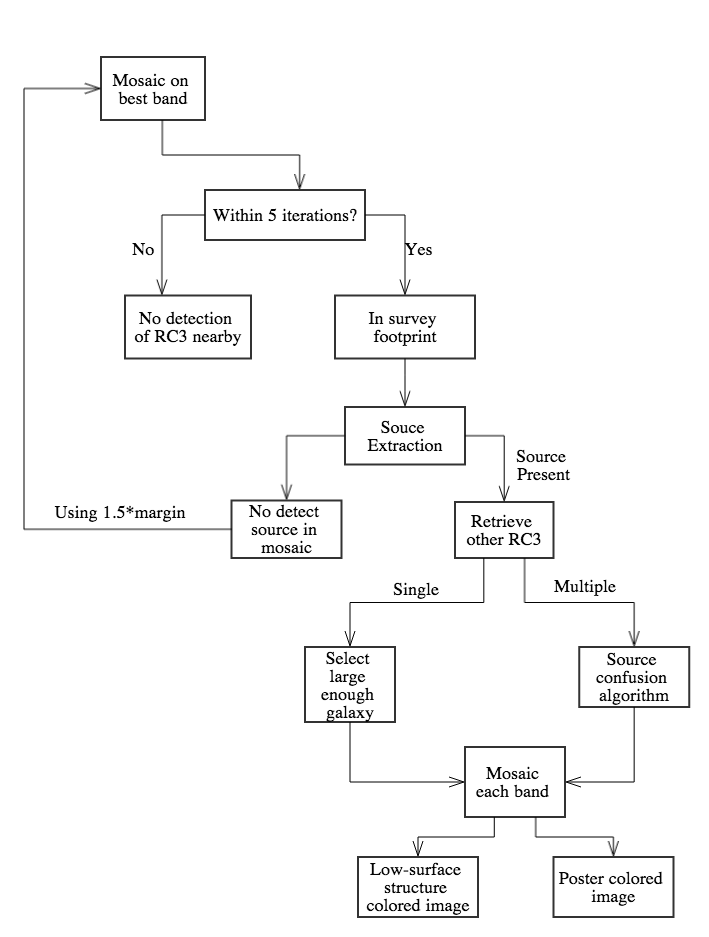
\includegraphics[width=0.5\textwidth]{figures/algorithm}
	\end{figure}
	\subsubsection{Positional Update} 
	To address the problem of inaccurate positions discussed in \autoref{sec:position}, we develop an algorithm that first updates the position by finding the galaxy in the imaging data. An  $\texttt{RC3}$ object contains its The Catalogue of Principal Galaxies(PGC) number, updated and catalog ra,dec,radius for each galaxy in the RC3 catalog. Since every RC3 galaxy has a unique PGC number, we record  its PGC number in order to identify the RC3 galaxy of interest for cases of source confusion and naming of data products. The method $\texttt{source\_info}$ updates the position of individual RC3 objects by first creating a single band mosaic with a field of view 6 times the radius of the galaxy, then SExtractor detects all sources in the mosaic and keeps only the ones with a radius greater than 5.94 arcseconds. This size cut is large enough such that it eliminates most stellar point sources and background noises  but retains the subset of RC2 galaxies inside the RC3 Catalog that are smaller than 1 arcminute as described by \citealp{rc2}. Also, if the mosaicking field is chosen correctly, then SExtractor's sky level estimation is fairly accurate.  
\\
\indent If there are multiple galaxies in the field of view that satisfy this criteria, then it is passed into the source confusion algorithm to determine the galaxy of interest. Then we record this single source and generate mosaic FITS file for all bands and color images using its updated values. If no sources are detected, then we mosaic the single band FITS using a larger field of view. This is done recursively, while keeping track of the number of iterations in each recursive steps. The process is terminated at the 3rd recursive step and generates a mosaic for all bands. Then we select mosaics from the three imaging bands  and recombine them to make two  colored mosaic. \label{sec:best_low}One emphasizes on low surface structures  so that the halos around the galaxy can be seen; the other image is a poster/publication image that uses higher cuts on the background to ensure a clean contrasting image. At least three band passes is necessary for generating a colored image since it enables R,G,B mapping by STIFF. Also, \citealp{2mass} explains that a minimum number of three bands  is required to distinguish the effects of interstellar extinction and stellar and extra-galactic populations, which is why many surveys has three imaging bands.
	\subsubsection{Source Confusion}
\begin{figure}
\begin{subfigure}{.2\textwidth}
\centering
  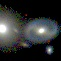
\includegraphics[width=.5\linewidth ]{figures/PGC58b4SC}
  \caption{Before}
\end{subfigure}%
%\hspace{-10pt}
\begin{subfigure}{.2\textwidth}
\centering
  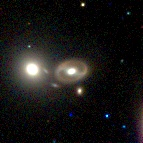
\includegraphics[width=.5\linewidth]{figures/PGC58afterSC}
  \caption{After} 
\end{subfigure}
\caption{ The three galaxies' arrangement is shown in \autoref{fig:positional_update_plot}. Using the source confusion algorithm, we resolve the three sources and generate recentered mosaic for PGC58.}
\label{fig:SCdemo}
\end{figure}
\indent Large galaxies tends to form gravitationally bound structure in clusters of galaxies. The source confusion algorithm works on the assumption that the only galaxies large enough to cause source confusion also lie in the RC3 catalog, since the catalog is reasonably complete for galaxies having apparent diameters larger than 1 arcminute. First, the program retrieves a list of n number of RC3 galaxies that may lie in the field of view of the generated mosaic. The $\texttt{otherRC3}$ method in the $\texttt{Server}$ class queries this information using the Vizier Catalog. If this information is provided by a survey's query service, such as the RC3 Table in SDSS's SkyServer, it can be overridden. The goal is to match the results returned by the server with the list of n largest sources detected by SExtractor. 
\\
\indent  We need to cross-correlate the coordinate by matching together the relative differences between the sources, due to the unreliability of absolute coordinates inherent to the catalog as discussed in section 2.1. We assume that the positional inaccuracy is due to  instrumentation and measurement error but retains the galaxies' locations relative to one another.  %no distortion that changes the relative positions among neighboring sources. 
Therefore, we compute all the possible distances between any two RC3 galaxies that lies in our field. Then compare this with the set of differences generated by the SExtractor-generated list. We select n number of galaxies that has the closest values in both list, thereby matching together the galaxies from the catalog  with the detected sources. Finally, we mosaic using that galaxy's coordinates as center. Our premises proves to be valid, as the algorithm executed with a success rate of 99.97\% in the SDSS run, and is capable of correctly resolving up to five RC3 sources in one example.
		\begin{figure}[h]
		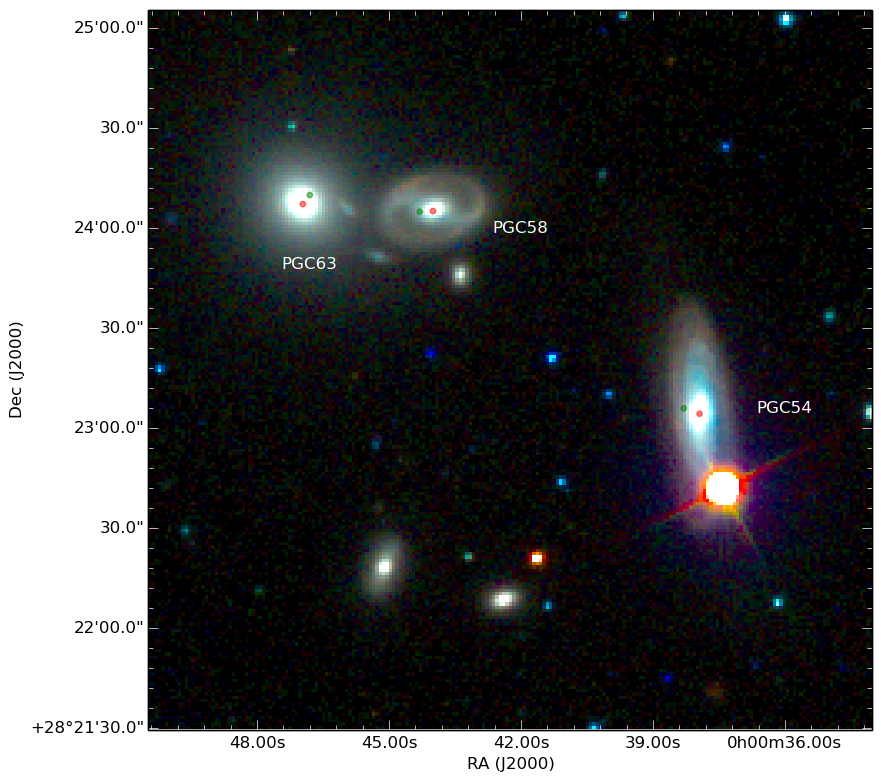
\includegraphics[width=0.5\textwidth]{figures/navigator}
		\caption{Three source confused RC3 Galaxies. Green marker denotes coordinates found in the original RC3 catalog, red marker denotes coordinates updated by the algorithm}
		\label{fig:positional_update_plot}
	\end{figure}
	\subsection{Pipeline}
	\begin{figure}[h]
		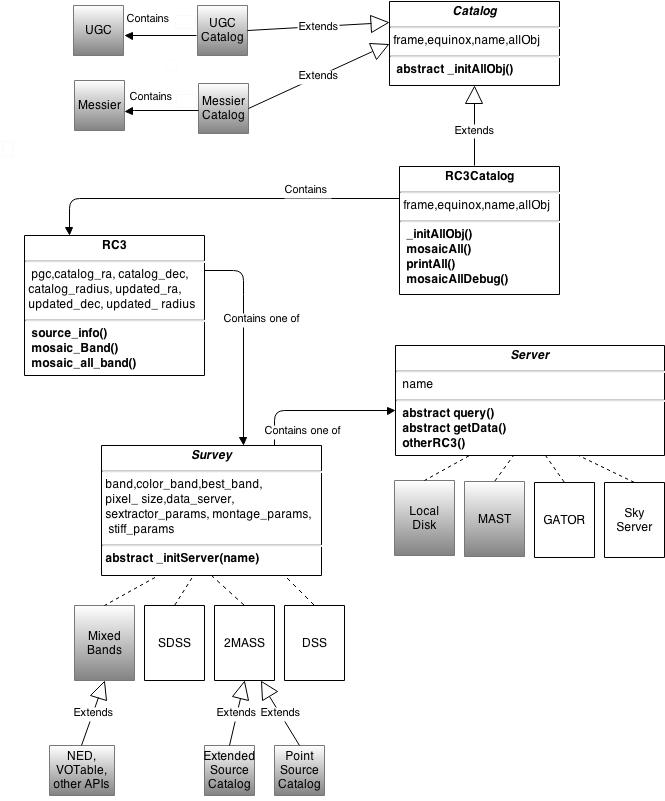
\includegraphics[width=0.5\textwidth]{figures/hierarchy}
		\label{fig:hierarchy}
		\caption{UML Class diagram showing the relationships in the mosaicking pipeline. Grey-filled boxes shows possible extensions of this pipeline}
	\end{figure}
 	The motivation behind building a class hierarchy is to establish a mosaicking pipeline for any given catalog and survey data. We identify the essential components required for mosaicking program to work. The relationship between these essential steps are reflected in our design of the abstract $\texttt{Survey}$, $\texttt{Catalog}$, and $\texttt{Server}$ classes. 
 		\subsubsection{Server}
		Data acquisition is composed of two main tasks: querying imaging data and retrieving data from server. Most surveys have an API that enables data access by SQL or customized query. To make the $\texttt{Server}$ class work, we need to figure out how to convert positional values to record-keeping parameters dependent on the survey's telescope. For example, SDSS image frames are uniquely identified by a particular combination of  run, camcol, and field and 2MASS refers to this with its sexagesimal, equatorial position-based source name. In the case where the survey has no special name referring to the imaging frame, such as in the case of POSS-II data, the user can invent their own naming scheme as placeholders for naming the raw imaging data. In addition to these two essential functions, each $\texttt{Server}$ class should also implement the query builder methods that are used inside the main mosaicking program.  Our choice of using a server instead of a data object enables code reusability across various surveys that uses common server tools , such as IPAC's GATOR query service (\citealp{irsa}) or  Astroquery.
	\subsubsection{Catalog Objects}
	For the purpose of mosaicking RC3 galaxies, we did not create a $\texttt{CatalogObject}$ class, although it would be helpful to have a generic class similar to the functions in $\texttt{RC3Objects}$ as an extension to the pipeline. They contain basic information about the particular object and are survey-independent. They perform the essential mosaicking features on a per-object basis so that they not only can be used for comparing resulting mosaics from multiple surveys (\autoref{fig:comparison}) but these methods can also be conventiently used in the $\texttt{Catalog}$ class. The final step in the mosaic procedure generates two TIFF color images as described in \autoref{sec:best_low}.  When extending the pipeline to other surveys, investigators can adjust the STIFF parameters to better suit the telescope-specific imaging details following the guidelines in \citealp{stiff}.
    \subsection{Catalog}
	The $\texttt{Catalog}$ class contains a list of objects that lies inside the catalog. Although the use of the $\texttt{Catalog}$ container class seems unnecessary, it enables a clear separation between basic mosaicking functionality for individual galaxies and for the entire catalog. This can be used to study some particular object, executed on all objects in a $\texttt{Catalog}$, or simply used for debugging purposes. This abstraction barrier ensures minimal changes to the code in both classes when an investigator decides to input data from a new survey in the future.
\section{Results}
\begin{figure*}[t!]
\centering
	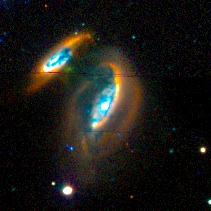
\includegraphics[width=0.3\textwidth]{figures/SDSS_120_LOW}
	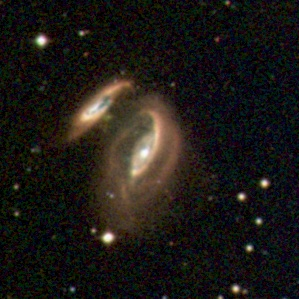
\includegraphics[width=0.3\textwidth]{figures/DSS_120_BEST}	
	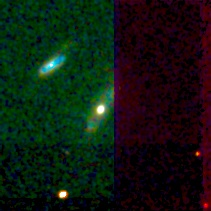
\includegraphics[width=0.3\textwidth]{figures/2MASS_120_BEST}
	\caption{PGC120 mosaic using SDSS, POSS-II, 2MASS data }
	\label{fig:comparison}
\end{figure*}
\subsection{Result from SDSS and DPOSS run}

\indent There are a total of 12512 RC3 galaxies within the SDSS footprint. The automated mosaicking pipeline was  successful for 90.22\% of the galaxies. 2446 RC3 galaxies is mosaicked using an updated position that was more than 1 arcminute off the values recorded in the RC3 catalog.  On a 8-core machine, the program processes on average about 80 RC3 objects per hour using SDSS data.  The finished data product occupies 39 GB of diskspace. 
\\
\indent  (\# More stats on this after DSS finishes its run) 
 For the POSS-II run, there are a total of [*] galaxies within the POSS-II footprint.
 The automated mosaicking pipeline was  successful for[*] \% of the galaxies. 2446 RC3 galaxies is mosaicked using an updated position that was more than 1 arcminute off the values recorded in the RC3 catalog. On the same machine that did the SDSS run, the program processes on average about 18.6 galaxies per hour using POSS-II data.  The finished data product occupies [*]GB of diskspace. 
\begin{figure}[h]
 \centering
	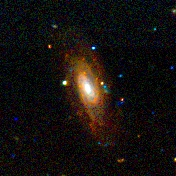
\includegraphics[width=0.2\textwidth]{figures/SDSS_1154_BEST}
	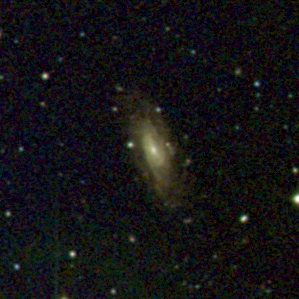
\includegraphics[width=0.2\textwidth]{figures/DSS_1154_BEST}	
	\caption{PGC1746 mosaic using SDSS and DSS}
	\label{sdss_dss_comp}
\end{figure}
	\subsection{Performance}	
	\indent We accelerate the mosaicking process by performing the recursive algorithm on only a single band FITS file designated as $\texttt{best\_band}$, then mosacking all bands only once per object. For SDSS, we use the image obtained by the r band filter since transmission curve in \citealp{edr} shows that r band has the highest quantum efficiency. For 2MASS, The $K_s$ band was chosen to be the $\texttt{best\_band}$ since it has the highest transmission as shown  in Figure 2 in \citealp{2mass}.
	\\
	 \indent  Most of the computation time is spent on downloading the raw FITS files from the survey's specific server. Therefore, even though Montage's modular design enables its performance to scale with number of processor  (\citealp{montage}), the process would not be significantly sped up by the use of Message Passing Interface (MPI). Therefore, the speed depends more on the data transfer rate between the host site and local machine rather than the number of cores in the machine. This average runtime would also depend on the sky coverage of the  particular survey and the speed of query.
	\\ \indent This process can  be significantly sped up if the investigator already has imaging data stored locally on a disk or have access to running the mosaic program alongside the survey's datacenter. We have designed our class hierarchy such that this can be written as a subclass of $\texttt{Server}$ with user-defined details of where the images are stored. However, it is not worthwhile to download the whole survey's imaging data set for this purpose since that would probably take more time than 
		\subsection{Technical Details}
		Due to the recent rise in popularity of Python usage in astronomy, we wrote the program in Python 2.7.6 so that the program's dependencies are more widely supported for extending its usage on future datasets. Most of the mosaic steps are done using IPAC's Montage  \citealp{montage} mosaic engine along with the AstroPy Montage wrapper\footnote{\url{http://www.astropy.org/montage-wrapper/}} and the final colored image is generated using Astromatic's STIFF v.2.4 \citealp{stiff}. Our choice of the two program makes use of the best features from each programs. Montage creates scientifically-calibrated images by retaining the astrometry and photometry of input sources during image reprojection step.STIFF provides the flexibility of adjusting many variables for the final colored image, as well as automatically estimating upper and lower cuts on the dynamic range using statistics derived from a pixel histogram. Most of the program interface requires building the URL query and parsing the resulting raw text or XML files downloaded by wget. Source extraction is done using SExtractor v.2.19.5 \citealp{sextractor}. The resulting web search database was created using the Python sqlite3 module and the web search interface was written in PHP with interacting HTML elements.
	\subsection{Known Errors}
	Even though a series of exception handling and error prevention mechanisms were put in place,  there are still errors in the data product that we produced. Error flags were put inside the web search database denoting the errors described below.
	\begin{verbatim}
			Error Information
			0 = no error
			1 = mosaicAll error
			2 = stiff error 
			3 = strange error
			4 = Montage image reprojection failure
			5= mSubImage failure
	\end{verbatim}
	 	\begin{enumerate}
	 	\item  mosaicAll error is a general error that is raised when the program breaks when mosaicking all bands.
	 	\item  STIFF  enforces that the mosaic FITS used for RGB mapping but must be exactly the same dimensions in order to generate a colored image. Sometimes no resulting color images produced because 3 colored band not the same size. This happens particularly more often in SDSS's g band and in DPOSS. %Not sure what this happens more in the g band specifically??
This also happens more often in DPOSS data since the photographic plates are non uniform in size. 
	 	\item  In the source confusion algorithm, we store the galaxies that pass the size cut inside a radius with PGC as key and position as values. This error flag is raised when SQL region search does not included the galaxy itself. 
	 	\item  $\texttt{mProjectExec}$ is the Montage procedure that creates the reprojected image from the raw FITS files. Sometimes reprojected images are not created even when Montages' debug statement clearly shows that the reprojection was successful and table and header files are corrupted. This results in an error in later mosaicking steps. We have implemented error prevention mechanism to ensure that mosaic procedures terminates correctly in such cases and wrote the problematic galaxy into failed\_projection, which can be examined later. 
	 	\item  $\texttt{mSubImage}$ crops a finished mosaic to the specified box frame. Montage throws an error when the program tries to crop the image with specified boundary lying outside the image field. We typically use a box length of two times the radius. If it doesn't work, another attempt for a smaller box size is made or the error is recorded. 
	 	\end{enumerate}	 
\indent Montage's background rectification module is not used in creating the FITS mosaics. Attempts were made in implementing these procedure, however it  is sometimes stuck in the step where the background model is applied to the projected images and  produces huge difference images files ($\approx$50GB) for reason that we have not figured out yet. This should not affect the astrometric quality of the data product. Sometimes scanlines may be seen as brightness differences in the SDSS mosaics, but the effect is much more severe and clear visible difference is  mostly  observed in the color images for 2MASS which manifests as distinct boundaries, and will likely affect the photometric quality of the resulting 2MASS mosaics.
 \section{Conclusion}
\indent Wide-area sky surveys are used to answer fundamental questions regarding large-scale structure and the cosmological history of the universe. The mosaicking pipeline described in this paper provides a convenient way to generate mosaics for sky survey imaging data for a given catalog, or on a per-image basis. This can be easily adapted for use on future data sets to create the scientifically-calibrated FITS mosaics as well as two colored images. We describe an algorithm that automatically updates the catalog using its inherently inaccurate positions and centers the galaxy around the newly updated coordinate for generating the mosaic. We generate a set of data product that resulted from running the RC3 catalog through the mosaicking pipeline using  SDSS and POSS-II data and  made this publically available through a searchable web form.
\\
\indent Feeding in the new data enables a greater  sky coverage and higher resolution images of objects inside the catalog, which can result in better astrometric and photometric results.  In addition, the pipeline can also be extended for other astronomical catalog such as the Messier Catalog or NGC, as well as user-defined catalogs. An investigator may define their own catalog by imposing selection limits to study a type of objects of interest. A text file containing positions, radius, and unique identifier for each object can be used as input to the pipeline. The scientifically calibrated FITS images can be used as for individual studies, as well as used for improved astrometry in updating the catalog position values. The multi-band FITS mosaics can also be combined with the calibrated mosaics of different wavelengths into multi-band color images with mosaics from single/double band surveys such as POSS-I and GALEX , if their image sizes are adjusted to match.  
\\
\indent The SDSS and POSS-II data product available on the LCDM website may also be useful  during  the target selection and commissioning stage of new surveying telescope such as the LSST and DECam. With the trend of future telescope having larger focal plane,, large nearby galaxies covered in the RC3 catalog needs to be properly masked to prevent the loss of imaging details from saturated CCDs. The updated RC3 coordinates tells us  which regions of the sky may be affected by these large galaxies, and the FITS files can be used to model-fit the galaxy's shape and light distribution. This information can also be used in selecting fiber location on spectroscopic targets that belong to the RC3 catalog. The FITS images can be used along with existing tools for scientific analysis, such as Astrometry.net(\citealp{astrometry.net}), SExtractor, APLpy(\citealp{aplpy}). The program is designed such that other APIs such as HEASARC's SkyView, Aladin, and NED can easily be latched on.
\\
\indent We have provided documentation on GitHub  that guides investigators through the steps to adapting the pipeline for future imaging data.The source code and documentation for the pipeline described in this paper can be found in the project repository: \url{https://github.com/ProfessorBrunner/rc3-sdss}. The data product from the SDSS and POSS-II run is available via a search form at \url{http://lcdm.astro.illinois.edu/search.html}.

\section*{Acknowledgements}
\footnotesize
\indent The work was supported by Google Summer of Code Program. We thank Harold G. Corwin, Jr. for helpful discussion that helped this work. This research made use of Montage, funded by the National Aeronautics and Space Administration's Earth Science Technology Office, Computation Technologies Project, under Cooperative Agreement Number NCC5-626 between NASA and the California Institute of Technology. Montage is maintained by the NASA/IPAC Infrared Science Archive. This research made use of Astropy, a community-developed core Python package for Astronomy (Astropy Collaboration, 2013).
\\
\indent  Funding for SDSS-III has been provided by the Alfred P. Sloan Foundation, the Participating Institutions, the National Science Foundation, and the U.S. Department of Energy Office of Science. The SDSS-III web site is http://www.sdss3.org/. SDSS-III is managed by the Astrophysical Research Consortium for the Participating Institutions of the SDSS-III Collaboration including the University of Arizona, the Brazilian Participation Group, Brookhaven National Laboratory, University of Cambridge, Carnegie Mellon University, University of Florida, the French Participation Group, the German Participation Group, Harvard University, the Instituto de Astrofisica de Canarias, the Michigan State/Notre Dame/JINA Participation Group, Johns Hopkins University, Lawrence Berkeley National Laboratory, Max Planck Institute for Astrophysics, Max Planck Institute for Extraterrestrial Physics, New Mexico State University, New York University, Ohio State University, Pennsylvania State University, University of Portsmouth, Princeton University, the Spanish Participation Group, University of Tokyo, University of Utah, Vanderbilt University, University of Virginia, University of Washington, and Yale University
\section*{References}
\bibliography{bibtex_database}
 %\bibliographystyle{abbrvnat}
%\bibliographystyle{apalike}
%\bibliographystyle{plainnat}
%\bibliographystyle{unsrtnat}
\bibliographystyle{elsarticle-harv}
\end{document}